% !TeX spellcheck = en_US

\chapter{Introduction}

	Everyone of us already had to deal with a defective consumer product. Years ago there was a good chance you could repair it by yourself. But with electronics getting more complex and integrated into nearly everything we own, this is becoming impossible.
	
	One of the best examples are laptops. They originated from a - by design - highly modular hardware system. Every part has a standardized connector that makes it possible to build up a computer out of components from various manufacturers. But due to market demand the devices had to shrink more and more. To cope with the hassle of little space, manufactures began to integrate these single components in one another. This greatly reduces the overall product size.
	
	\begin{figure}[H]
		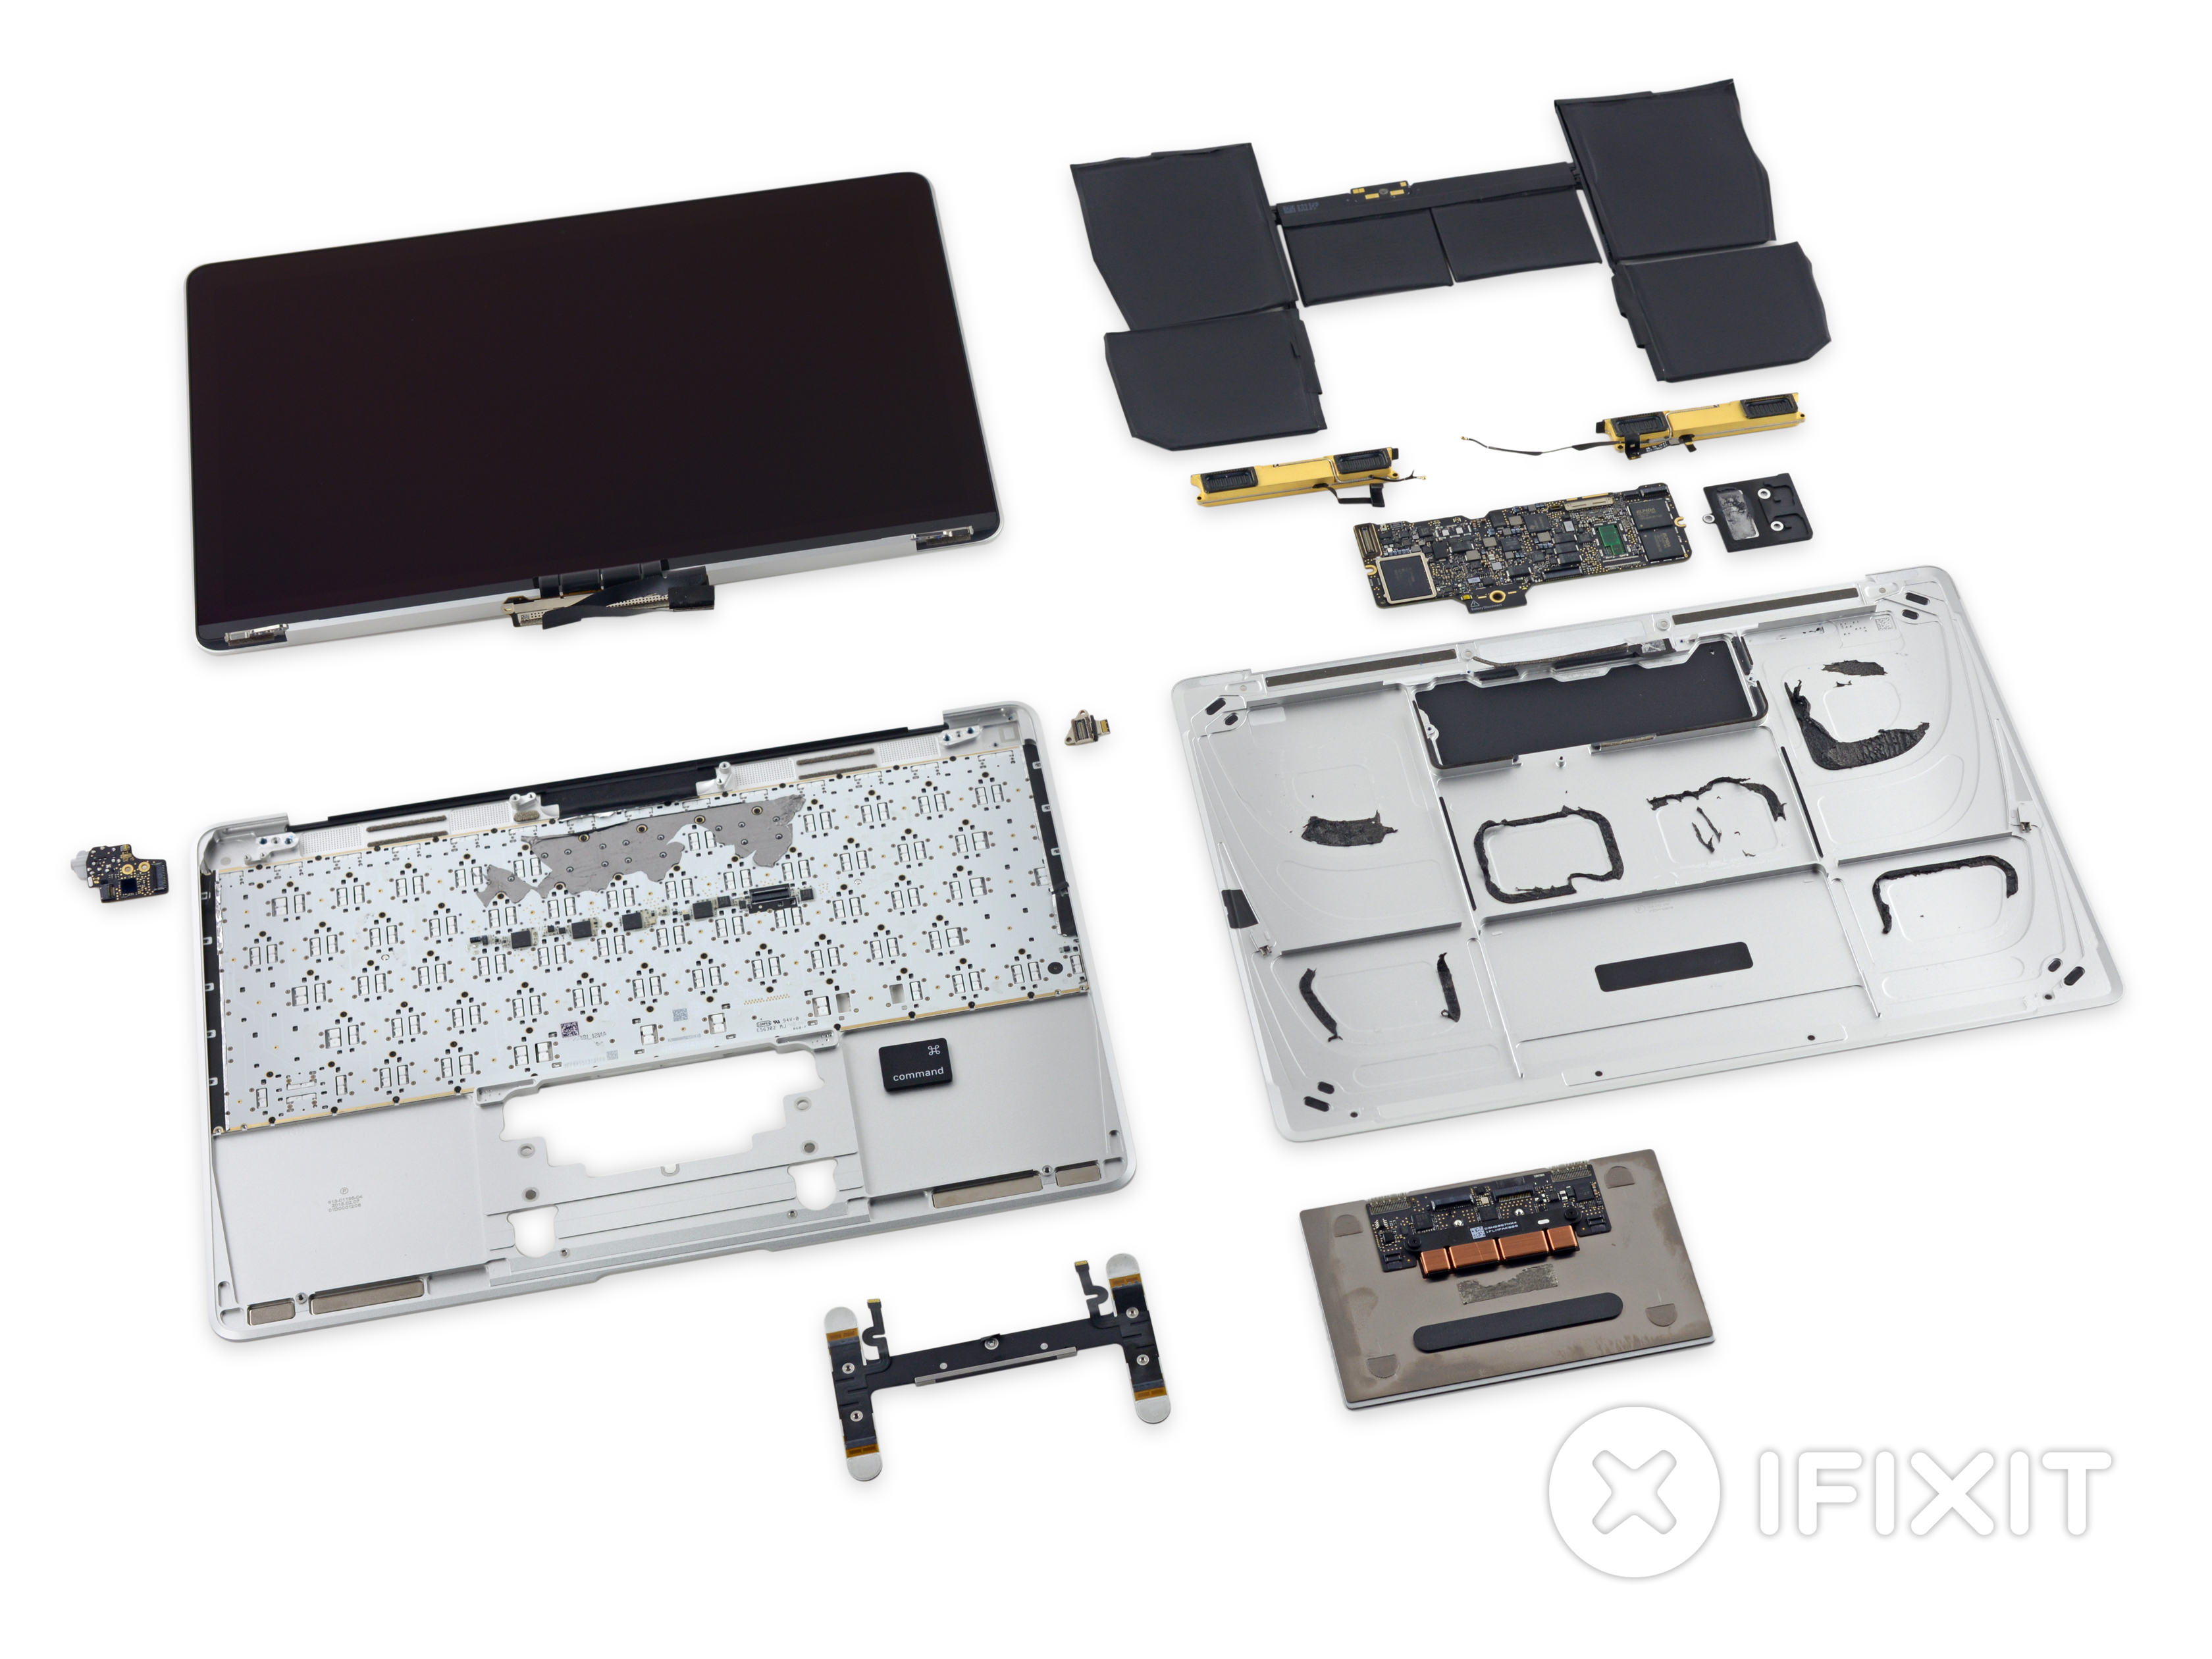
\includegraphics[width=\textwidth]{../images/ifixit-macbook-parts.jpg}
		\centering
		\caption[Disassembled Apple MacBook 2015 that got a iFixit Repairability Score of 1 out of 10]{Disassembled Apple MacBook 2015 that got a iFixit Repairability Score of 1 out of 10\footnotemark}
		\label{fig:ifixit-macbook-parts}
	\end{figure}
	\footnotetext{\url{https://de.ifixit.com/Teardown/Retina+MacBook+2015+Teardown/39841}}
	
	The most recent achievement of these politics can be seen in \autoref{fig:ifixit-macbook-parts}. The Apple MacBook 2015 is extremely thin which led the engineers few possibilities regarding the size of the electronics. Contradicting the traditional modular idea, everything from CPU to flash memory is soldered onto one single circuit board. It can only be replaced as one expensive part, but only if this is possible at all. The use of special adhesive saves the space needed for screws, yet it is not possible to handle for an end user.
	
	Of course this is not limited to mobile computer hardware. In almost every industry products become less and less fixable. Where 30 years ago you could repair your car by replacing the broken part in a straightforward way, nowadays you do not even know whats defective without the help of professionals.
	
	\begin{figure}[H]
		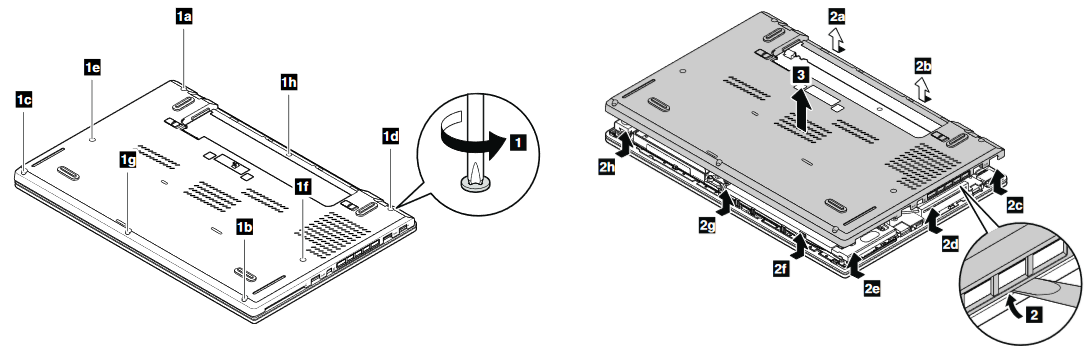
\includegraphics[width=\textwidth]{../images/common-manual.png}
		\centering
		\caption[Typical step-by-step manual for business laptop hardware, taken from Hardware Maintainance Manual by Lenovo Thinkpad]{Typical step-by-step manual for business laptop hardware, taken from Hardware Maintainance Manual by Lenovo Thinkpad\footnotemark}
		\label{fig:lenovo-hardware-manual}
	\end{figure}
	\footnotetext{\url{https://download.lenovo.com/ibmdl/pub/pc/pccbbs/mobiles_pdf/t440s_hmm_en_sp40a25360_04.pdf}}
	
	\textit{Furthermore the manufacturers do not want you to refurbish a product. They want you as the end user to buy new things.}
	
	Solely the business sector demands products that are serviceable. \autoref{fig:lenovo-hardware-manual} shows an excerpt from a hardware maintenance manual for a professional business notebook by Lenovo. Almost all parts of this laptop are replaceable when following the instructions. But creating this manual, providing spare parts for end users and most importantly design the product in a way it can be easily fixed are pretty expensive. This effort will be omitted with consumer products.
	
	\paragraph{So what can you do?}

	solution:
	\begin{itemize}
		\itemsep0em
		\item find a professional (expensive)
		\item repair the thing yourself \begin{itemize}
			\itemsep0em
			\item with the help of the manufacture \begin{itemize}
				\item not really wanted > a repaired product last longer and shrinks profits from selling new product
				\item nowadays only for professional equipment (business laptops, ...)
					
					\begin{figure}[H]
						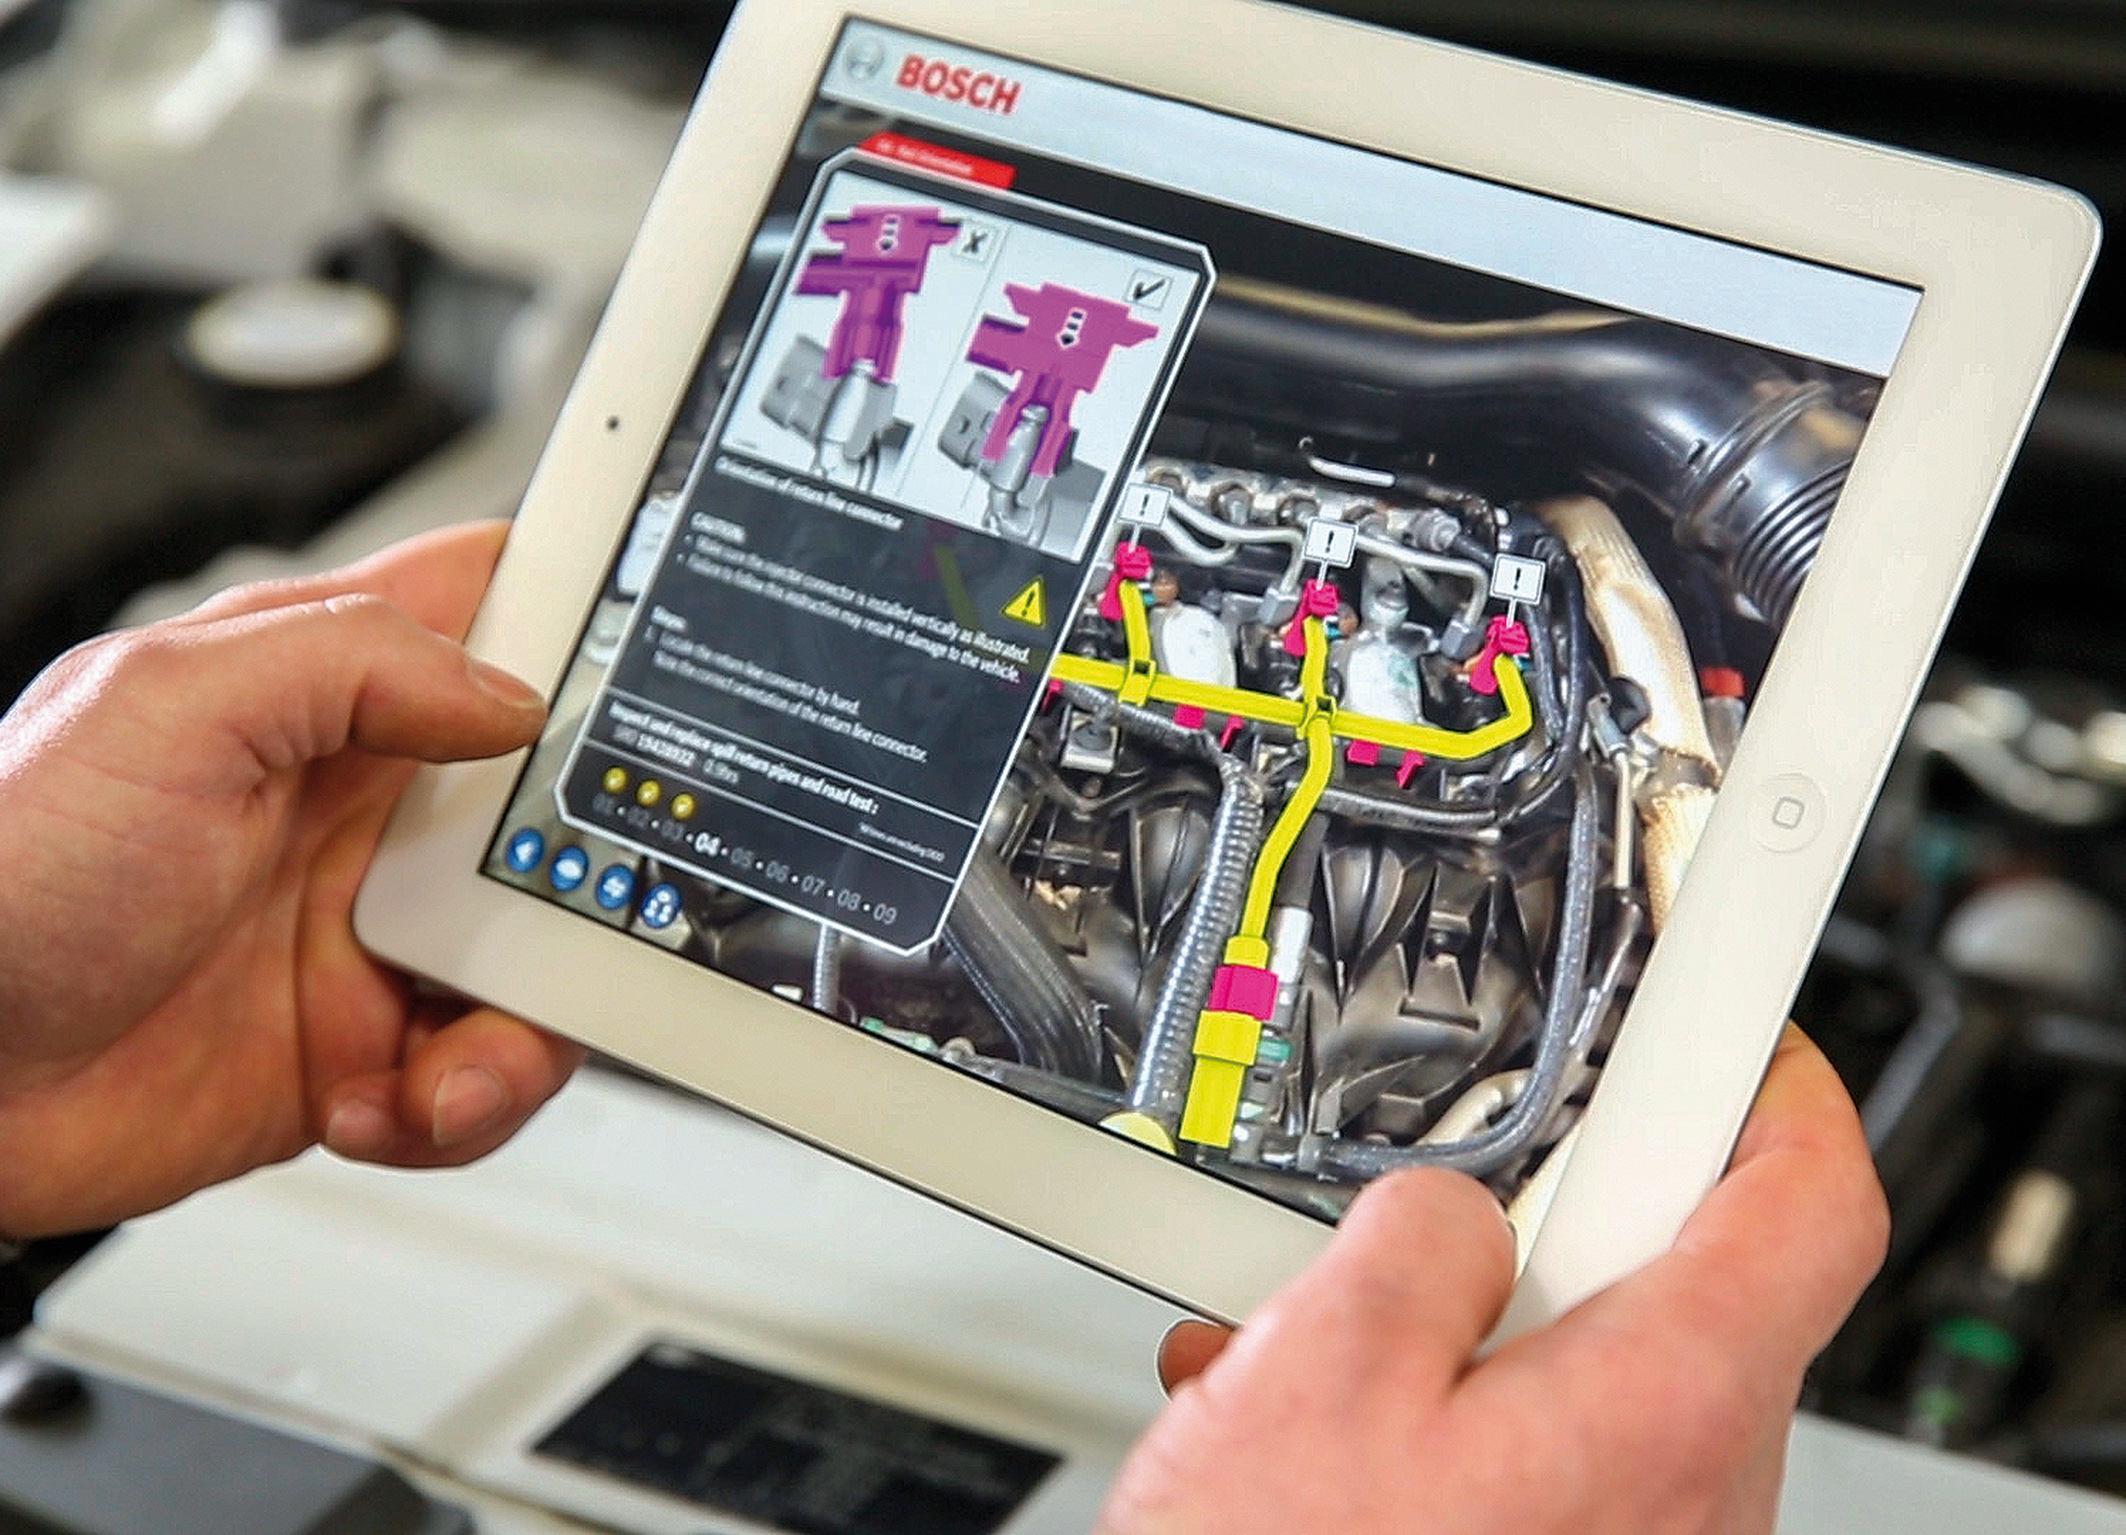
\includegraphics[width=0.9\textwidth]{../images/bosch-flex-inspect.jpg}
						\centering
						\caption[Professional augmented reality equipment by Bosch designed to help the repair shop personal]{Professional augmented reality equipment by Bosch designed to help the repair shop personal\footnotemark}
					\end{figure}
					\footnotetext{\url{http://www.bosch-presse.de/presseforum/details.htm?txtID=6938&tk_id=109}}
			\end{itemize}
			\item without the help of the manufacture \begin{itemize}
				\itemsep0em
				\item with technical skills > requirements increase drastically
				\item with no technical skills > manuals by other users (youtube videos, ...)
			\end{itemize}
			\begin{figure}[H]
				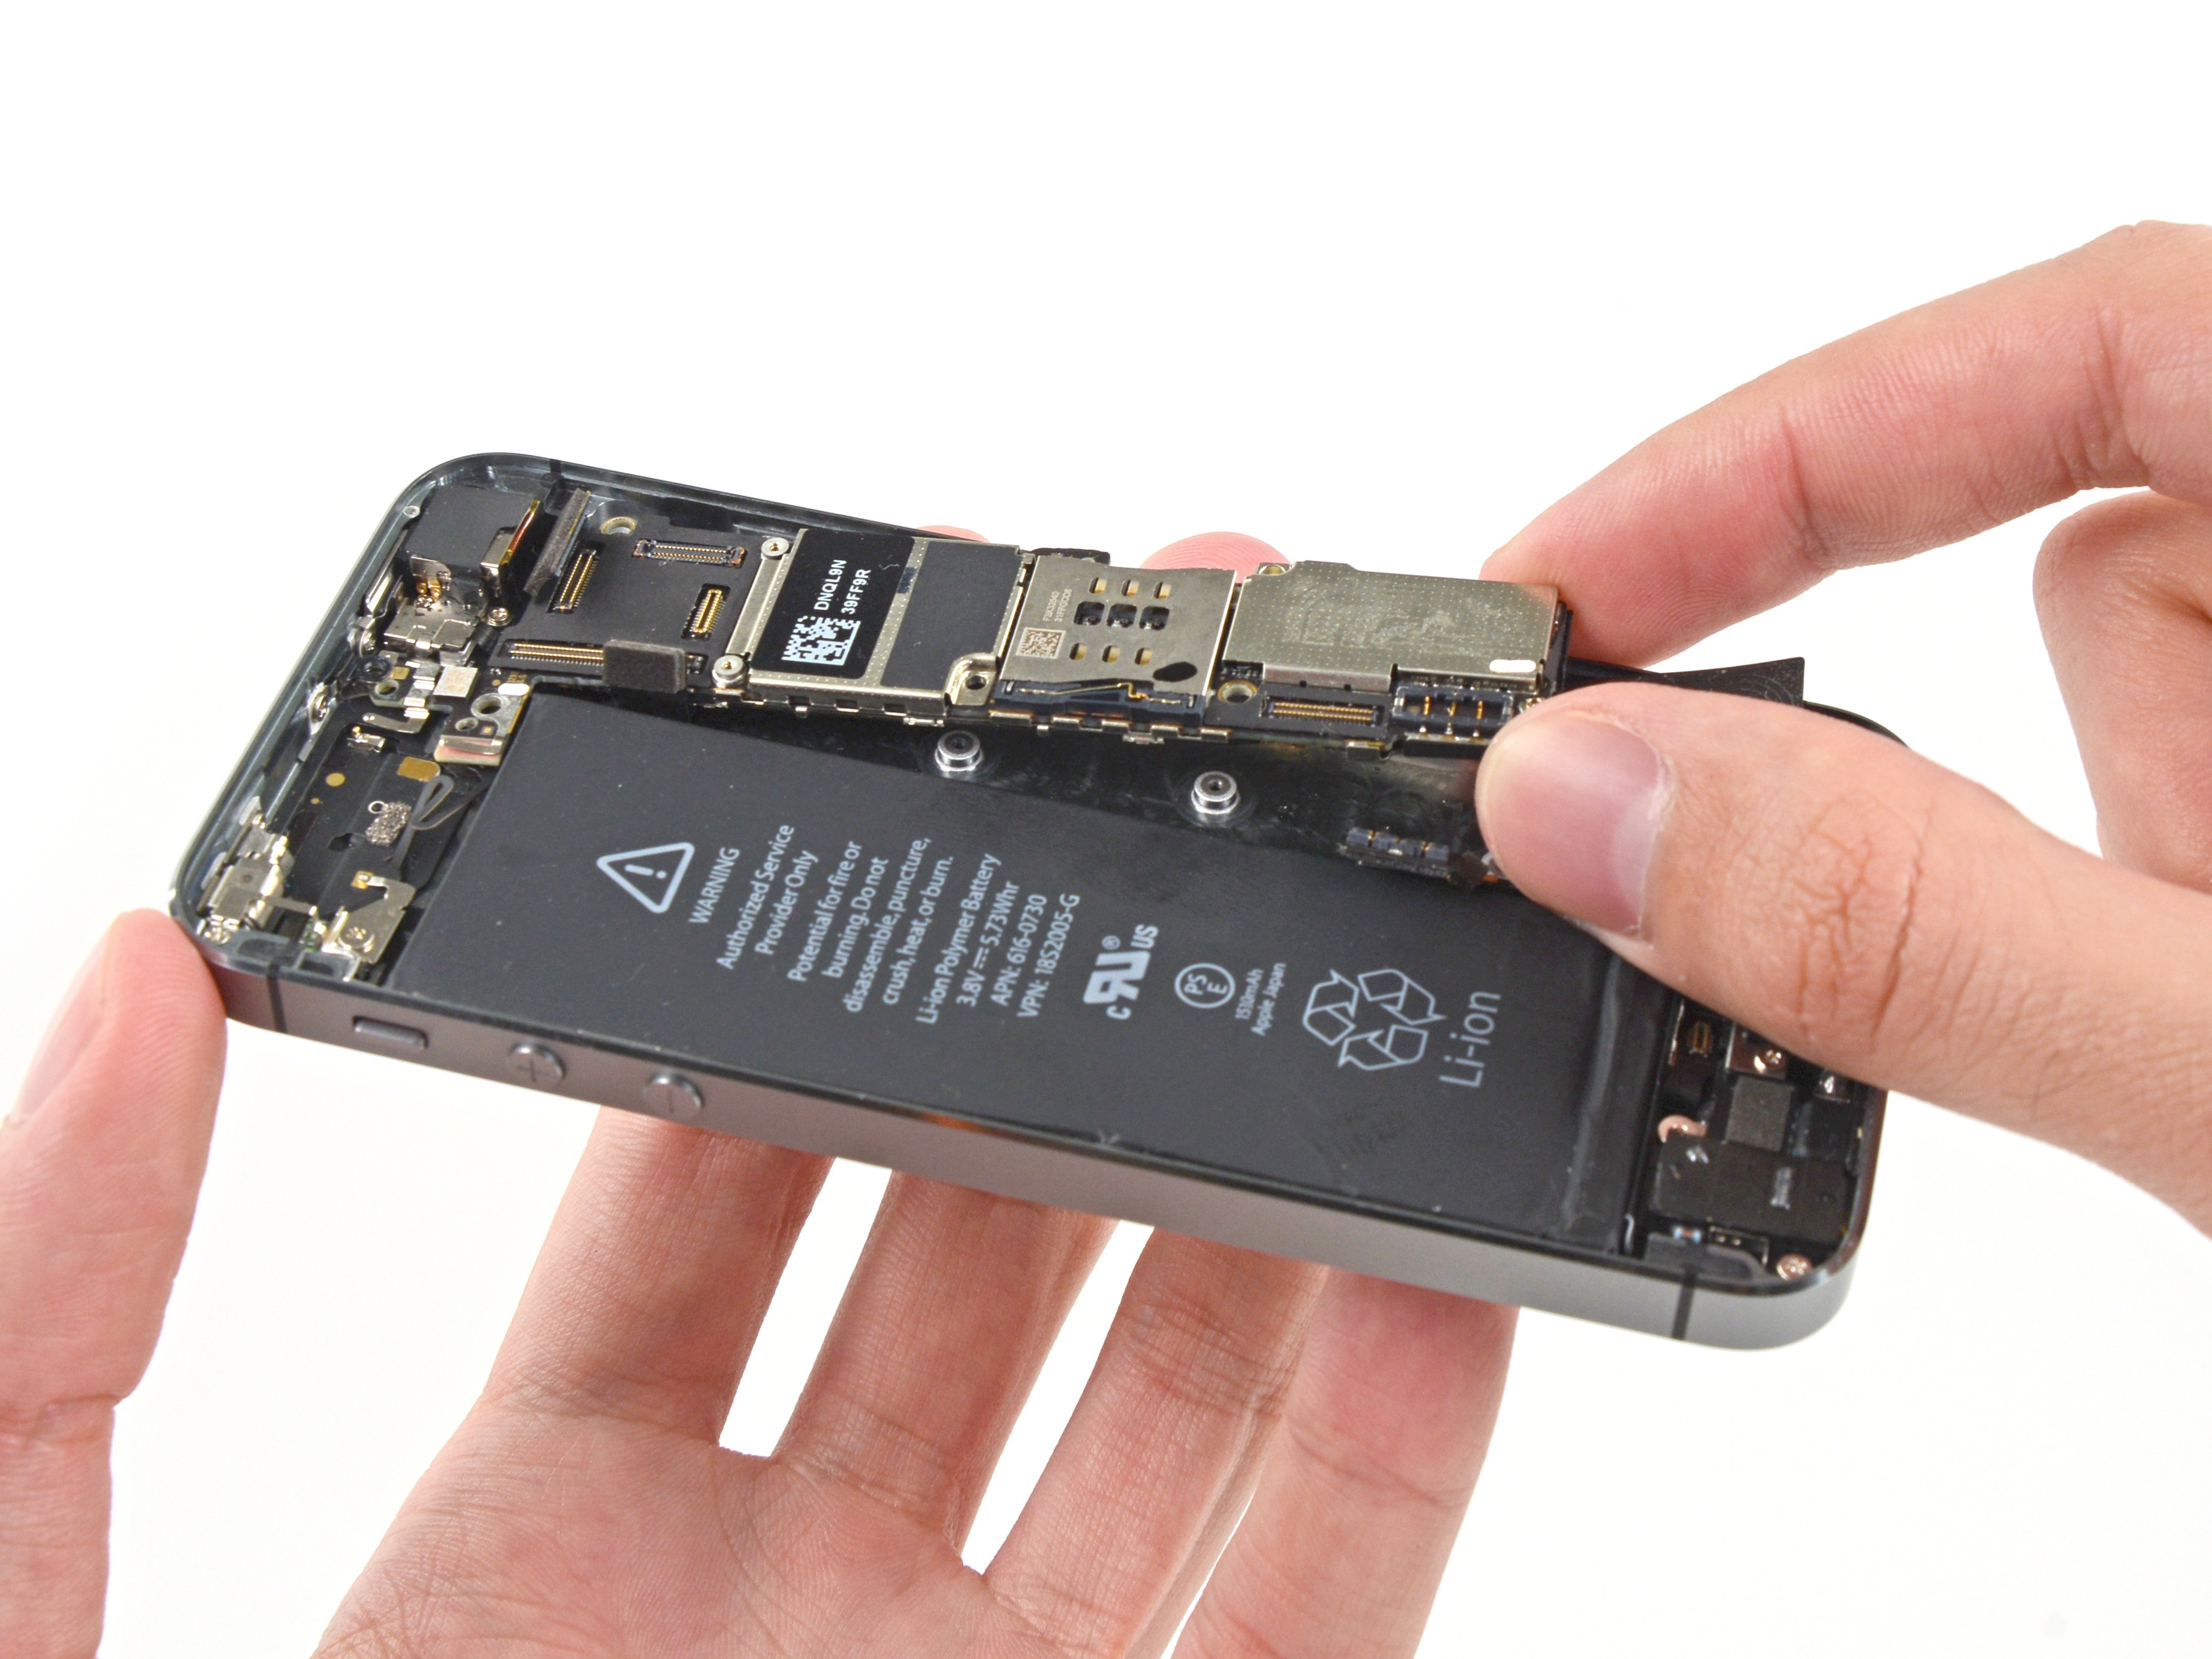
\includegraphics[width=0.8\textwidth]{../images/ifixit-iphone-logicboard.jpg}
				\centering
				\caption[Single step taken from an iFixit repair manual for replacing the iPhone5 logic board]{Single step taken from an iFixit repair manual for replacing the iPhone5 logic board\footnotemark}
			\end{figure}
			\footnotetext{\url{https://de.ifixit.com/Guide/id/20246}}
		\end{itemize}
	\end{itemize}
	
	OUR solution:
	\begin{itemize}
		\itemsep0em
		\item \textbf{help user with repairing things by their own}
		\item new approach: use AR
		\item AR will come into the houses over the next years > device available
		\item AR devices are designed to show/add information to your environment and at the same time keep your hands free (alternation and interaction possible!) (not for tablets, ...) ...
	\end{itemize}
	
	
	section 2 will deal with the general product idea.
	
	section 3 takes a look at the specific problems that have to be faced because we use augmented reality
	
	section 4 checks possible business opportunities

